\documentclass[10.5pt]{article}

% -------------------- Page and typography --------------------
\usepackage[paper=a4paper,margin=0.78in,top=0.72in,bottom=0.82in]{geometry}
\usepackage[T1]{fontenc}
\usepackage[utf8]{inputenc}
\usepackage{newtxtext,newtxmath}
\usepackage[tracking=true,protrusion=true,expansion=true]{microtype}
\usepackage{setspace}
\setstretch{1.06}
\usepackage{parskip}
\setlength{\parskip}{5.5pt}
\setlength{\parindent}{0pt}
\usepackage{enumitem}
\setlist{nosep,leftmargin=1.35em}
\usepackage{booktabs,tabularx,array,multirow}
\usepackage{amsmath}
\let\openbox\relax
\usepackage{amsthm,mathtools}
\usepackage{graphicx}
\usepackage{float}
\usepackage{caption}
\usepackage{subcaption}
\usepackage{tikz}
\usetikzlibrary{arrows.meta,positioning,calc,fit,shapes.geometric,shapes.misc,backgrounds,matrix,decorations.pathmorphing}
\usepackage[most]{tcolorbox}
\usepackage{titlesec}
\usepackage{fancyhdr}
\usepackage{lastpage}
\usepackage{hyperref}
\usepackage{xcolor}
\usepackage{fontawesome5}
\usepackage{algorithm2e}
\setlength{\headheight}{20pt}
\sloppy

% -------------------- Colors --------------------
\definecolor{goInk}{HTML}{10131A}
\definecolor{goNavy}{HTML}{001B4C}
\definecolor{goBlue}{HTML}{2147A8}
\definecolor{goViolet}{HTML}{5B3FFF}
\definecolor{goCyan}{HTML}{00A9C8}
\definecolor{goGold}{HTML}{B98222}
\definecolor{goGoldLight}{HTML}{F6E8C8}
\definecolor{goGreen}{HTML}{1C8C5A}
\definecolor{goRed}{HTML}{B6424B}
\definecolor{goPaper}{HTML}{FDFBF6}
\definecolor{goPale}{HTML}{F4F7FB}
\definecolor{goLine}{HTML}{C9D8EF}
\definecolor{goGraph}{HTML}{EDE9FF}

\pagecolor{goPaper}
\color{goInk}
\hypersetup{colorlinks=true,linkcolor=goBlue,citecolor=goBlue,urlcolor=goBlue,pdfauthor={Vincent Boucher},pdftitle={GoalOS: The Validated Skill Graph}}

% -------------------- Header/footer --------------------
\pagestyle{fancy}
\fancyhf{}
\fancyhead[L]{\footnotesize\scshape GoalOS: The Validated Skill Graph}
\fancyhead[R]{\footnotesize\scshape Vincent Boucher \;|\; QUEBEC.AI \& MONTREAL.AI}
\renewcommand{\headrulewidth}{0.3pt}
\renewcommand{\headrule}{\hbox to\headwidth{\color{goGold}\leaders\hrule height \headrulewidth\hfill}}
\fancyfoot[C]{\footnotesize\color{goNavy}\thepage\,/\,\pageref*{LastPage}}

% -------------------- Section style --------------------
\titleformat{\section}{\Large\bfseries\scshape\color{goNavy}}{\thesection}{0.65em}{}
\titleformat{\subsection}{\large\bfseries\color{goNavy}}{\thesubsection}{0.6em}{}
\titleformat{\subsubsection}{\normalsize\bfseries\color{goNavy}}{\thesubsubsection}{0.5em}{}
\titlespacing*{\section}{0pt}{12pt}{3pt}
\titlespacing*{\subsection}{0pt}{9pt}{2pt}
\captionsetup{font=small,labelfont={bf,color=goNavy},textfont=it,skip=4pt}

% -------------------- Theorem boxes --------------------
\newtheoremstyle{goThm}%
{7pt}{7pt}{\itshape}{} {\bfseries\color{goNavy}}{.}{0.5em}{}
\theoremstyle{goThm}
\newtheorem{definition}{Definition}
\newtheorem{proposition}{Proposition}
\newtheorem{principle}{Principle}

% -------------------- TColor boxes --------------------
\tcbset{enhanced,boxrule=0.4pt,arc=3mm,left=7pt,right=7pt,top=6pt,bottom=6pt}
\newtcolorbox{thesisbox}{colback=goNavy!3,colframe=goGold!65!black,borderline west={1.2pt}{0pt}{goGold},sharp corners=downhill}
\newtcolorbox{policybox}{colback=goBlue!3,colframe=goBlue!35!goNavy}
\newtcolorbox{warningbox}{colback=goRed!3,colframe=goRed!55!black,borderline west={1.2pt}{0pt}{goRed}}

% -------------------- TikZ styles --------------------
\tikzset{
  arr/.style={-{Latex[length=2.2mm,width=1.5mm]}, line width=0.55pt, draw=goViolet},
  arr2/.style={-{Latex[length=2mm,width=1.3mm]}, line width=0.48pt, draw=goGold!85!black, dashed},
  arrg/.style={-{Latex[length=2mm,width=1.3mm]}, line width=0.55pt, draw=goGreen!85!black},
  arrr/.style={-{Latex[length=2mm,width=1.3mm]}, line width=0.55pt, draw=goRed!85!black},
  nodebox/.style={rounded corners=6pt, draw=goBlue!40, fill=white, very thin, align=center, minimum height=9mm, inner sep=4pt, font=\footnotesize},
  nodepale/.style={rounded corners=6pt, draw=goViolet!45, fill=goGraph!55, very thin, align=center, minimum height=9mm, inner sep=4pt, font=\footnotesize},
  gate/.style={diamond, aspect=2.35, draw=goGold!75!black, fill=goGoldLight!55, line width=0.45pt, align=center, inner sep=2pt, font=\footnotesize\bfseries},
  greenbox/.style={rounded corners=6pt, draw=goGreen!60!black, fill=goGreen!6, very thin, align=center, minimum height=9mm, inner sep=4pt, font=\footnotesize},
  redbox/.style={rounded corners=6pt, draw=goRed!65!black, fill=goRed!5, very thin, align=center, minimum height=9mm, inner sep=4pt, font=\footnotesize},
  goldbox/.style={rounded corners=6pt, draw=goGold!70!black, fill=goGoldLight!35, very thin, align=center, minimum height=9mm, inner sep=4pt, font=\footnotesize},
  skill/.style={circle, draw=goViolet!60, fill=goGraph!40, line width=0.45pt, align=center, minimum size=19mm, inner sep=2pt, font=\scriptsize},
  plate/.style={draw=goLine, rounded corners=9pt, fill=white, line width=0.4pt}
}

\newcommand{\vsg}{\textsc{Validated Skill Graph}}
\newcommand{\chronicle}{\textsc{Chronicle}}
\newcommand{\goalos}{\textsc{GoalOS}}
\newcommand{\pb}{\textsc{ProofBundle}}
\newcommand{\ed}{\textsc{Evidence Docket}}
\newcommand{\job}{\textsc{AGI Job}}
\newcommand{\jobs}{\textsc{AGI Jobs}}

\begin{document}

% -------------------- Title page --------------------
\begin{titlepage}
\centering
\vspace*{0.45in}
{\Huge\bfseries\color{goInk} GoalOS: The Validated Skill Graph\par}
\vspace{0.18in}
{\Large\itshape\color{goNavy} Reusable Capability, Chronicle-Gated Memory, and Proof-Carrying Skill Accumulation\par}
\vspace{0.16in}
{\color{goGold}\rule{0.26\textwidth}{0.5pt}\hspace{0.8em}$\star$\hspace{0.8em}\rule{0.26\textwidth}{0.5pt}\par}
\vspace{0.25in}
{\large Vincent Boucher\par}
{\normalsize President, QUEBEC.AI \& MONTREAL.AI\par}
\vspace{0.2in}
{\small Montreal.AI Research \;|\; July 2026\par}

\vspace{0.42in}
\begin{thesisbox}
\large\textbf{Thesis.} The durable asset in an autonomous proof economy is not a prompt, a transcript, or a polished model answer. It is a \emph{validated skill}: a scoped, replayable, evidence-backed capability object that has survived proof, validation, risk checks, and \chronicle{} admission. The \vsg{} is the institutional memory layer that stores and compounds those capabilities.
\end{thesisbox}

\vfill
\begin{figure}[H]
\centering
\resizebox{0.98\textwidth}{!}{%
\begin{tikzpicture}[x=1cm,y=1cm]
  \node[plate, minimum width=16.5cm, minimum height=6.0cm] (p) at (0,0) {};
  \node[nodebox, minimum width=2.3cm] (o) at (-6.4,1.7) {\faBullseye\\Objective};
  \node[nodebox, minimum width=2.35cm] (m) at (-3.3,1.7) {Mission\\Contract};
  \node[goldbox, minimum width=2.2cm] (d) at (-0.4,1.7) {Proof\\Debt};
  \node[nodepale, minimum width=2.35cm] (j) at (2.6,1.7) {Custom\\AGI Jobs};
  \node[nodebox, minimum width=2.15cm] (b) at (5.4,1.7) {Proof\\Bundles};
  \node[nodebox, minimum width=2.35cm] (e) at (5.4,-0.3) {Evidence\\Docket};
  \node[gate, minimum width=2.0cm] (g) at (2.6,-0.3) {Chronicle\\Gate};
  \node[greenbox, minimum width=2.5cm] (s) at (-0.4,-0.3) {Validated\\Skill Node};
  \node[greenbox, minimum width=2.55cm] (vg) at (-3.3,-0.3) {Validated\\Skill Graph};
  \node[nodebox, minimum width=2.45cm] (f) at (-6.4,-0.3) {Future Mission\\Influence};
  \draw[arr] (o) -- (m);
  \draw[arr] (m) -- (d);
  \draw[arr] (d) -- (j);
  \draw[arr] (j) -- (b);
  \draw[arr] (b) -- (e);
  \draw[arr] (e) -- (g);
  \draw[arrg] (g) -- (s);
  \draw[arrg] (s) -- (vg);
  \draw[arrg] (vg) -- (f);
  \draw[arr2] (f.north) .. controls (-6.4,3.0) and (-6.4,3.0) .. (o.north) node[midway,left,align=center,font=\scriptsize\color{goGold!70!black}] {validated capability\\selects harder missions};
  \node[goldbox, minimum width=2.65cm] (h) at (2.6,-2.1) {Mainnet Handoff\\Packet};
  \draw[arr2] (j) -- (h);
  \node[align=left,font=\scriptsize\color{goInk}] at (5.3,-2.1) {Live posting, escrow, bonds, disputes,\\and settlement remain outside local mode.};
  \draw[arr2] (h) -- (4.0,-2.1);
\end{tikzpicture}}
\caption{The \vsg{} transforms validated outcomes into reusable capability. Drafting creates candidates; proof work creates evidence; \chronicle{} admits only validated skill.}
\end{figure}
\vfill
{\footnotesize\color{goNavy}This paper is a publication-safe, claim-bounded architecture and product research edition. It does not claim achieved AGI, ASI, empirical SOTA, legal certification, investment advice, live wallet support, or production authorization.}
\end{titlepage}

\section{Abstract}
\goalos{} treats language-model output as candidate material, not institutional memory. A model can propose a plan, draft an argument, or produce a workflow, but those artifacts should not automatically shape future behavior. This paper isolates one layer of the \goalos{} architecture: the \vsg{}, a governed memory substrate for reusable capability. The graph stores only skills that have passed an explicit admission process: proof debt is retired, \pb{}s are returned, an \ed{} aggregates and tests the evidence, the \chronicle{} Gate evaluates the configured proof level, and only then does a capability become reusable memory. The resulting graph is not a prompt library. It is a typed, versioned, scoped, replayable, provenance-backed network of capability objects. We formalize the skill-node object model, edge semantics, proof-level-dependent admission, repair paths through custom \jobs{}, skill composition, worth-keeping utility, threat model, evaluation program, and commercial implications. The central contribution is a memory discipline for autonomous work: what compounds is not output volume, but validated reusable capability.

\section{Introduction}
The first wave of AI products made generation cheap. They produced answers, drafts, code, plans, reports, and summaries. But institutions cannot govern themselves with persuasive text alone. They require a reliable answer to a harder question: which outputs deserve reuse, trust, propagation, settlement, and future influence?

The \vsg{} answers that question by separating \emph{candidate output} from \emph{validated capability}. A skill is admitted only after an evidence path exists. A reusable capability is not a sentence, a prompt, or a transcript; it is a proof-carrying operational object with provenance, scope, acceptance tests, replay instructions, risk boundaries, and measured utility.

This paper focuses only on that layer. It assumes the broader \goalos{} operating loop: objective, mission contract, autonomous work, verification, \ed{}, governed decision state, action graph, \chronicle{}, and reusable capability. Mission OS defines this as a proof-to-action system in which the user supplies an objective and \goalos{} runs until proof is done \cite{goalosMissionOS}. AEP-001 states the constitutional boundary: private intelligence remains off-chain, while proof commitments, attestations, and evolution rights can be governed; no proof, no evolution; no evaluation, no propagation; no rollback, no release \cite{aep001}.

\begin{thesisbox}
\textbf{Positioning.} A prompt repository stores instructions. A transcript archive stores conversation. A vector database stores recallable fragments. The \vsg{} stores validated capability: what worked, under which constraints, with which evidence, for which scope, and with which proof level.
\end{thesisbox}

\section{Problem: Memory Without Proof}
Autonomous systems become dangerous or unreliable when memory is too permissive. A system that remembers every confident output can compound errors, overclaims, stale evidence, reward hacks, and unsupported assumptions. This creates four failure modes.

\begin{enumerate}[label=\textbf{F\arabic*.}]
  \item \textbf{Contagious unsupported claims.} A persuasive answer enters memory and influences later missions without proof.
  \item \textbf{Prompt-library drift.} Useful instructions are copied and reused outside the context where they were valid.
  \item \textbf{Invisible provenance loss.} Future operators cannot determine what evidence justified a prior capability.
  \item \textbf{Ungated self-improvement.} The system treats successful-sounding behavior as improvement, even when it has not passed replay, risk, or validation checks.
\end{enumerate}

The \vsg{} is a countermeasure. It creates a narrow bridge from output to memory. Nothing becomes durable merely because it is well-written. Memory is earned through evidence.

\section{Definitions}

\begin{definition}[Candidate Work]
Candidate work is any draft, plan, code fragment, analysis, workflow, claim, artifact, or agent trace produced before \chronicle{} admission. Candidate work may be useful, but it has no durable memory authority.
\end{definition}

\begin{definition}[Proof Debt]
Proof debt is an explicit record of missing evidence required before a claim, artifact, or capability can be trusted at the selected proof level. Proof debt is retired by evidence, review, replay, test results, or other accepted proof artifacts.
\end{definition}

\begin{definition}[Validated Skill]
A validated skill is a scoped capability object admitted by the \chronicle{} Gate after its proof debt is sufficiently retired. A validated skill includes scope, preconditions, evidence, replay instructions, risk boundaries, version metadata, and usage policy.
\end{definition}

\begin{definition}[Validated Skill Graph]
The \vsg{} is a typed directed multigraph whose nodes are validated skills and whose edges encode reuse, composition, teaching, packaging, audit, repair, retirement, and future mission influence.
\end{definition}

\section{System Positioning}
The \vsg{} lives at the boundary between proof and memory. Figure~\ref{fig:substrate} shows the governed transition from candidate work to reusable capability.

\begin{figure}[H]
\centering
\resizebox{\textwidth}{!}{%
\begin{tikzpicture}[x=1cm,y=1cm]
  \node[plate, minimum width=17.2cm, minimum height=8.1cm] (plate) at (0,0) {};
  \node[align=center,font=\footnotesize\bfseries\color{goNavy}] at (-6.2,3.35) {1. Candidate Work};
  \node[align=center,font=\footnotesize\bfseries\color{goNavy}] at (-2.1,3.35) {2. Proof Economy};
  \node[align=center,font=\footnotesize\bfseries\color{goNavy}] at (2.1,3.35) {3. Chronicle Gate};
  \node[align=center,font=\footnotesize\bfseries\color{goNavy}] at (6.1,3.35) {4. Validated Memory};

  \node[nodebox, minimum width=2.15cm] (draft) at (-6.2,2.4) {LLM Draft\\candidate output};
  \node[nodebox, minimum width=2.15cm] (claims) at (-6.2,1.25) {Claim Extraction\\atomic assertions};
  \node[goldbox, minimum width=2.15cm] (debt) at (-6.2,0.1) {Proof Debt\\unsupported items};
  \draw[arr2] (draft) -- (claims);
  \draw[arr2] (claims) -- (debt);

  \node[nodepale, minimum width=2.35cm] (jobs) at (-2.1,1.9) {Custom\\AGI Jobs};
  \node[nodebox, minimum width=2.35cm] (bundles) at (-2.1,0.75) {ProofBundles};
  \node[nodebox, minimum width=2.35cm] (docket) at (-2.1,-0.4) {Evidence\\Docket};
  \draw[arr] (debt.east) -- (jobs.west);
  \draw[arr] (jobs) -- (bundles);
  \draw[arr] (bundles) -- (docket);

  \node[gate, minimum width=2.45cm] (gate) at (2.1,0.75) {Selection\\Gate};
  \node[greenbox, minimum width=2.2cm] (admit) at (2.1,2.0) {Admit\\skill node};
  \node[goldbox, minimum width=2.2cm] (repair) at (2.1,-0.6) {Repair\\create jobs};
  \draw[arr] (docket.east) -- (gate.west);
  \draw[arrg] (gate) -- (admit);
  \draw[arr2] (gate) -- (repair);
  \draw[arr2] (repair.west) -- (debt.east);

  \node[skill] (core) at (6.1,0.8) {Validated\\Skill\\Graph};
  \foreach \ang/\name in {90/Reuse,30/Compose,-30/Teach,-90/Package,-150/Audit,150/Replay}{
    \node[skill, minimum size=15mm] (n\ang) at ($(core)+(\ang:1.75)$) {\name};
    \draw[arrg] (core) -- (n\ang);
    \draw[arrg] (n\ang) -- (core);
  }
  \draw[arrg] (admit.east) .. controls (4.0,2.2) and (4.7,1.3) .. (core.north west);
  \node[goldbox, minimum width=3.1cm] (future) at (0,-2.65) {Future Mission Influence\\only from admitted skills};
  \draw[arr2] (core.south) .. controls (5.5,-2.3) and (2.2,-2.65) .. (future.east);
  \draw[arr2] (future.west) .. controls (-3.4,-2.65) and (-6.6,-1.2) .. (debt.south);

  \node[goldbox, minimum width=13.2cm, font=\footnotesize\itshape] at (0,-3.55) {LLMs may draft; only proof-admitted skills persist. Failed candidates repair proof debt, not memory.};
\end{tikzpicture}}
\caption{\vsg{} as a governed memory substrate. Candidate output becomes durable capability only after proof and \chronicle{} admission.}
\label{fig:substrate}
\end{figure}

\section{Formal Object Model}
Let a skill node be represented by
\begin{equation}
  s = (id, type, scope, L, P, E, V, R, B, U, \tau, \rho),
\end{equation}
where \(id\) is a stable identifier, \(type\) is the skill class, \(scope\) is its permitted operating domain, \(L\) is the proof level, \(P\) is the proof-debt ledger, \(E\) is the evidence set, \(V\) is validator coverage, \(R\) is replay material, \(B\) is the risk boundary, \(U\) is utility telemetry, \(\tau\) is version and lineage metadata, and \(\rho\) is the rollback or retirement policy.


\begin{figure}[H]
\centering
\resizebox{0.98\textwidth}{!}{%
\begin{tikzpicture}[x=1cm,y=1cm]
  \node[plate, minimum width=16.5cm, minimum height=7.0cm] at (0,0) {};
  \node[greenbox, minimum width=3.55cm, minimum height=1.6cm, font=\large\bfseries] (core) at (0,0) {Validated Skill Node\\\footnotesize proof-carrying reusable capability};
  \node[nodebox, minimum width=3.0cm] (scope) at (-5.2,2.4) {\textbf{Scope}\\\scriptsize domain, authority, prohibited uses};
  \node[nodebox, minimum width=3.0cm] (tests) at (-1.75,2.4) {\textbf{Acceptance Tests}\\\scriptsize objective, metrics, verifier rubric};
  \node[nodebox, minimum width=3.0cm] (proof) at (1.75,2.4) {\textbf{Proof Level}\\\scriptsize L1--L5 admission policy};
  \node[nodebox, minimum width=3.0cm] (evidence) at (5.2,2.4) {\textbf{Evidence}\\\scriptsize ProofBundles, reviews, docket};
  \node[nodebox, minimum width=3.0cm] (lineage) at (-5.2,-2.4) {\textbf{Lineage}\\\scriptsize parent nodes, version, rollback};
  \node[nodebox, minimum width=3.0cm] (replay) at (-1.75,-2.4) {\textbf{Replay Manifest}\\\scriptsize inputs, tools, constraints};
  \node[nodebox, minimum width=3.0cm] (risk) at (1.75,-2.4) {\textbf{Risk Boundary}\\\scriptsize safety, legal, settlement limits};
  \node[nodebox, minimum width=3.0cm] (utility) at (5.2,-2.4) {\textbf{Utility Telemetry}\\\scriptsize reuse, time saved, quality delta};
  \foreach \n in {scope,tests,proof,evidence,lineage,replay,risk,utility}{\draw[arr] (\n) -- (core);}
  \node[goldbox, minimum width=14.1cm, font=\footnotesize\itshape] at (0,-3.25) {A skill node is not a note or prompt. It is a bounded operational object with proof, replay, risk, utility, and rollback.};
\end{tikzpicture}}
\caption{Skill-node passport. Every admitted node carries operational identity, evidence, replay, risk, utility, and rollback metadata.}
\label{fig:node-passport}
\end{figure}


\begin{table}[H]
\centering
\caption{Canonical skill-node fields.}
\label{tab:nodefields}
\begin{tabularx}{\textwidth}{>{\bfseries\color{goNavy}}p{0.22\textwidth}X}
\toprule
Field & Function \\
\midrule
Scope & Defines where the capability may be reused; prevents domain drift. \\
Proof level & Binds the node to an admission standard from exploratory through formal. \\
Evidence & Links to \pb{}s, \ed{} entries, reviews, replay logs, and source commitments. \\
Acceptance tests & Specifies what must be true before the node is considered valid. \\
Validator coverage & Records reviewer or AGI Node attestations and unresolved dissent. \\
Replay manifest & Enables reproduction or reconstruction of the capability path. \\
Risk boundary & States safety, legal, policy, settlement, and operational constraints. \\
Utility telemetry & Records observed reuse, quality, time saved, error rate, and mission impact. \\
Rollback policy & Specifies retirement, repair, quarantine, and version reversion triggers. \\
\bottomrule
\end{tabularx}
\end{table}

\section{Chronicle Admission Policy}
The \chronicle{} Gate is the memory firewall. It decides whether a candidate skill becomes durable capability, requires repair, or is rejected. Let \(A_L(s)\in\{0,1\}\) denote admission at proof level \(L\). A simple admission rule is
\begin{equation}
A_L(s)=1 \quad\Longleftrightarrow\quad
\begin{cases}
\operatorname{support}(s)\ge \theta^{support}_L,\\
\operatorname{replay}(s)\ge \theta^{replay}_L,\\
\operatorname{validation}(s)\ge \theta^{validation}_L,\\
\operatorname{risk}(s)\le \theta^{risk}_L,\\
\operatorname{scope\_ok}(s)=1. 
\end{cases}
\end{equation}
The thresholds are policy parameters. Raising proof level increases the evidence burden and reduces the chance that persuasive but ungrounded material enters memory.

\begin{figure}[H]
\centering
\resizebox{0.94\textwidth}{!}{%
\begin{tikzpicture}[x=1cm,y=1cm]
  \node[plate, minimum width=15.6cm, minimum height=6.3cm] at (0,0) {};
  \node[nodebox, minimum width=2.7cm] (cand) at (-6.1,0.6) {Candidate\\Skill};
  \node[nodebox, minimum width=2.8cm] (docket) at (-2.9,0.6) {Evidence\\Docket};
  \node[gate, minimum width=2.2cm] (gate) at (0.5,0.6) {Chronicle\\Gate};
  \node[greenbox, minimum width=2.7cm] (admit) at (4.2,2.0) {Admit\\memory entry};
  \node[goldbox, minimum width=2.7cm] (repair) at (4.2,0.55) {Repair\\create AGI Jobs};
  \node[redbox, minimum width=2.7cm] (reject) at (4.2,-1.0) {Reject /\\Quarantine};
  \node[nodepale, minimum width=2.65cm] (support) at (-2.9,2.0) {Support\\strength};
  \node[nodepale, minimum width=2.65cm] (replay) at (-2.9,-1.0) {Replay\\path};
  \node[nodepale, minimum width=2.65cm] (valid) at (0.5,2.0) {Validation\\coverage};
  \node[nodepale, minimum width=2.65cm] (risk) at (0.5,-1.0) {Risk\\posture};
  \draw[arr] (cand) -- (docket);
  \draw[arr] (docket) -- (gate);
  \draw[arr] (support) -- (docket);
  \draw[arr] (replay) -- (docket);
  \draw[arr] (valid) -- (gate);
  \draw[arr] (risk) -- (gate);
  \draw[arrg] (gate) -- (admit);
  \draw[arr2] (gate) -- (repair);
  \draw[arrr] (gate) -- (reject);
  \draw[arr2] (repair.west) .. controls (0.7,-2.0) and (-4.8,-1.7) .. (cand.south);
  \node[goldbox, minimum width=13.3cm, font=\footnotesize\itshape] at (-1.0,-2.55) {Gate law: admission requires support, replay, validation, risk posture, and scope compatibility at the configured proof level. Repair creates jobs for missing proof; rejection does not modify memory.};
\end{tikzpicture}}
\caption{Chronicle admission policy. Evidence becomes authority only when it satisfies the selected proof level.}
\label{fig:chronicle}
\end{figure}

\section{Flexible Proof Levels}
Different work requires different proof. A brainstorming session, an internal playbook, a public claim, a mainnet handoff, and a production-grade memory entry should not share the same admission threshold. \goalos{} therefore treats proof level as a first-class mission parameter.

\begin{table}[H]
\centering
\caption{Proof levels for skill admission.}
\label{tab:prooflevels}
\begin{tabularx}{\textwidth}{>{\bfseries}p{0.08\textwidth}p{0.22\textwidth}X X}
\toprule
Level & Name & Required evidence posture & Memory effect \\
\midrule
L1 & Structural / Demo & Mission structure, explicit proof debt, local artifact coherence. & No durable \chronicle{} influence. \\
L2 & Internal Review & Operator confirms usefulness, scope, and risk boundaries. & Temporary reuse, clearly labeled. \\
L3 & External Review & Independent reviewer, AGI Node validation, or cross-source corroboration. & Scoped reusable skill. \\
L4 & Mainnet Handoff & Validated evidence, job specification, settlement boundary, and explicit handoff packet. & Skill may inform external execution preparation. \\
L5 & Chronicle / Formal & Multi-validator evidence, replay, baseline comparison, risk gate, and rollback condition. & Durable skill with future mission influence. \\
\bottomrule
\end{tabularx}
\end{table}

\begin{figure}[H]
\centering
\resizebox{0.96\textwidth}{!}{%
\begin{tikzpicture}[x=1cm,y=1cm]
  \node[plate, minimum width=16cm, minimum height=6.2cm] at (0,0) {};
  \node[align=center,font=\bfseries\color{goNavy}] at (-5.8,2.55) {Proof-Level Ladder};
  \foreach \i/\lab/\desc/\y/\col in {
    1/L1 Demo/structure only/1.6/goGreen,
    2/L2 Internal/operator reviewed/0.8/goCyan,
    3/L3 External/independent review/0.0/goViolet,
    4/L4 Handoff/settlement packet/-0.8/goGold,
    5/L5 Formal/replay + rollback/-1.6/goRed}{
    \node[circle, minimum size=7mm, draw=\col!70!black, fill=\col!12, font=\footnotesize\bfseries] at (-7.0,\y) {\i};
    \node[align=left,font=\footnotesize] at (-5.6,\y) {\textbf{\lab}\\\scriptsize \desc};
  }
  \node[align=center,font=\bfseries\color{goNavy}] at (-1.1,2.55) {Operational Effects};
  \foreach \x/\head in {-2.7/Job granularity,-0.9/Validators,0.9/Evidence,2.7/Chronicle}{
    \node[align=center,font=\scriptsize\bfseries\color{goNavy}] at (\x,1.75) {\head};
  }
  \foreach \r/\y in {1/1.1,2/0.45,3/-0.2,4/-0.85,5/-1.5}{
    \foreach \c/\x in {1/-2.7,2/-0.9,3/0.9,4/2.7}{
      \pgfmathtruncatemacro{\dots}{min(5,\r+\c-1)}
      \node[align=center,font=\scriptsize\color{goViolet}] at (\x,\y) {\foreach \k in {1,...,\dots}{\textbullet\ }};
    }
  }
  \node[align=center,font=\bfseries\color{goNavy}] at (5.7,2.55) {Admission Policy};
  \node[greenbox, minimum width=3.2cm] at (5.7,1.15) {Low rigor\\fast learning};
  \node[goldbox, minimum width=3.2cm] at (5.7,0.0) {Medium rigor\\reviewed reuse};
  \node[redbox, minimum width=3.2cm] at (5.7,-1.15) {High rigor\\durable memory};
  \draw[arr] (-4.2,-2.35) -- (4.1,-2.35) node[midway,below,font=\scriptsize\color{goNavy}] {increasing proof cost, validation burden, and memory authority};
\end{tikzpicture}}
\caption{Proof-level policy. The selected level calibrates job design, validator burden, evidence strictness, and memory authority.}
\label{fig:prooflevels}
\end{figure}

\section{Graph Semantics}
The \vsg{} is a directed typed multigraph \(G_t=(S_t,E_t)\). Each edge is a tuple
\begin{equation}
  e=(s_i, \rho, s_j, w, C, \pi),
\end{equation}
where \(s_i\) and \(s_j\) are skill nodes, \(\rho\) is the relation type, \(w\) is an observed utility or confidence weight, \(C\) is the context in which the relation has been observed, and \(\pi\) is evidence provenance.

\begin{table}[H]
\centering
\caption{Core graph relations.}
\label{tab:edges}
\begin{tabularx}{\textwidth}{>{\bfseries\color{goNavy}}p{0.18\textwidth}p{0.28\textwidth}X}
\toprule
Relation & Meaning & Example \\
\midrule
Reuse & Skill applies in a new mission context. & A reviewer-room pattern used for a new AI vendor diligence mission. \\
Compose & Skills combine into a higher-order capability. & Claim-boundary skill + job-design skill = proof-mission factory. \\
Teach & Skill can train operators or agents. & A validated review heuristic becomes a Masterclass lesson. \\
Package & Skill is converted into a product artifact. & A proof packet becomes an AI Trust Room template. \\
Audit & Skill requires periodic review or risk checks. & A compliance-related skill is revalidated when policies change. \\
Retire & Skill is deprecated, superseded, or quarantined. & A skill fails replay or becomes unsafe outside its original scope. \\
Influence & Skill reduces uncertainty in future mission planning. & Validated evidence reduces proof debt in a related mission. \\
\bottomrule
\end{tabularx}
\end{table}


\begin{figure}[H]
\centering
\resizebox{0.98\textwidth}{!}{%
\begin{tikzpicture}[x=1cm,y=1cm]
  \node[plate, minimum width=16.8cm, minimum height=7.0cm] at (0,0) {};
  \node[skill, minimum size=22mm] (vp) at (-5.8,1.6) {Vision\\to Proof};
  \node[skill, minimum size=22mm] (rr) at (-3.3,2.3) {Reviewer\\Judgment};
  \node[skill, minimum size=22mm] (dr) at (-0.8,2.3) {Domain\\Research};
  \node[skill, minimum size=24mm] (jd) at (-2.0,0.3) {Job\\Design};
  \node[skill, minimum size=22mm] (rp) at (-4.0,-1.65) {Replay\\Practice};
  \node[skill, minimum size=22mm] (ba) at (0.4,-1.65) {Boundary\\Audit};
  \node[skill, minimum size=22mm] (pk) at (2.55,0.3) {Packaging\\Templates};
  \draw[arr] (vp) -- node[above,font=\scriptsize] {compose} (jd);
  \draw[arrg] (rr) -- node[above,font=\scriptsize] {audit} (jd);
  \draw[arr] (dr) -- node[right,font=\scriptsize] {evidence} (jd);
  \draw[arrg] (jd) -- node[left,font=\scriptsize] {teach} (rp);
  \draw[arr2] (ba) -- node[below,font=\scriptsize] {risk check} (jd);
  \draw[arr] (jd) -- node[above,font=\scriptsize] {package} (pk);
  \draw[arr2] (pk.south) .. controls (1.3,-3.0) and (-4.8,-2.9) .. (vp.south) node[midway,below,font=\scriptsize\color{goGold!70!black}] {future mission influence};
  \node[goldbox, align=left, minimum width=5.6cm, font=\footnotesize] at (5.3,1.35) {\textbf{Edge law}\\Each edge carries relation type, context, provenance, observed utility, and expiry conditions. Edges weaken or retire when replay fails, risk rises, or usefulness decays.};
  \node[nodebox, align=left, minimum width=5.6cm, font=\footnotesize] at (5.3,-1.45) {\textbf{Operations}\\Reuse: apply in new scope.\\Compose: build higher-order skill.\\Teach: derive lesson or rubric.\\Package: ship proof room or job template.\\Audit/Retire: protect memory quality.};
\end{tikzpicture}}
\caption{Graph semantics. Validated skills are connected by typed, evidence-carrying operations rather than informal similarity.}
\label{fig:edges}
\end{figure}


\section{Skill Capture Studio}
The Skill Capture Studio converts expert judgment into candidate skills. The objective is not to memorize a meeting or imitate an expert style; it is to isolate reusable operations that can be validated.

\begin{enumerate}[label=\textbf{S\arabic*.}]
  \item \textbf{Extract episodes.} Identify concrete expert moves: framing, critique, boundary-setting, repair, evaluation, packaging.
  \item \textbf{Create candidate nodes.} Assign type, scope, proof level, and first-pass utility hypothesis.
  \item \textbf{Generate proof debt.} Record what evidence would be needed before reuse is safe.
  \item \textbf{Create custom jobs.} Convert unresolved proof into \jobs{} with worker roles, validators, and acceptance tests.
  \item \textbf{Admit or repair.} Use the \chronicle{} Gate to determine whether the capability becomes durable memory.
\end{enumerate}

\section{Worth-Keeping Utility}
Not every validated artifact should become a durable skill. Memory can bloat. The graph therefore needs a worth-keeping function that trades off value, reuse, cost, risk, and maintenance burden. One practical score is
\begin{equation}
W(s) = \alpha V(s) + \beta R_u(s) + \gamma Q(s) - \lambda C_p(s) - \mu Risk(s) - \nu M(s),
\end{equation}
where \(V\) is observed value, \(R_u\) is reuse potential, \(Q\) is quality or validation strength, \(C_p\) is proof cost, \(Risk\) is residual risk, and \(M\) is maintenance burden. A skill is retained only if
\begin{equation}
A_L(s)=1 \quad \text{and} \quad W(s) > \theta^{keep}_{type,scope}.
\end{equation}

\begin{policybox}
\textbf{Worth-keeping principle.} A skill should enter durable memory only when its expected future utility exceeds its proof cost, risk, and maintenance burden. Passing proof is necessary; being worth keeping is an additional economic and governance test.
\end{policybox}

\section{Capability Composition}
Skill composition is powerful because it turns atomic capabilities into higher-order capabilities. It is also dangerous because composition may amplify risk. Therefore two or more skills may compose only when their scopes, assumptions, evidence levels, and risk boundaries are compatible.

\begin{proposition}[Composition Gate]
Let \(S_C=\{s_1,\dots,s_n\}\) be a candidate composition. The composite skill \(s_C\) may enter the graph only if each component is admitted, the composition proof level is at least the maximum required level of the output scope, and the joint risk remains under policy threshold:
\begin{equation}
A(s_C)=1 \Rightarrow \bigwedge_{i=1}^{n} A(s_i)=1, \quad L(s_C) \ge \max_i L(s_i), \quad Risk(S_C)\le \theta_{C}.
\end{equation}
\end{proposition}

\begin{figure}[H]
\centering
\resizebox{0.95\textwidth}{!}{%
\begin{tikzpicture}[x=1cm,y=1cm]
  \node[plate, minimum width=15.9cm, minimum height=6.0cm] at (0,0) {};
  \node[skill] (a) at (-5.4,1.1) {Claim\\Boundary};
  \node[skill] (b) at (-5.4,-1.1) {Reviewer\\Rubric};
  \node[skill] (c) at (-2.7,1.1) {Evidence\\Mapping};
  \node[skill] (d) at (-2.7,-1.1) {Job\\Design};
  \node[gate, minimum width=2.4cm] (gate) at (0.3,0) {Composition\\Gate};
  \node[greenbox, minimum width=2.8cm] (comp) at (3.4,0.8) {Proof Mission\\Factory Skill};
  \node[redbox, minimum width=2.8cm] (fail) at (3.4,-0.9) {Repair /\\Reject};
  \node[goldbox, minimum width=3.1cm] (tests) at (6.2,0.8) {New tests:\\scope, replay, risk};
  \foreach \n in {a,b,c,d}{\draw[arr] (\n) -- (gate);}
  \draw[arrg] (gate) -- (comp);
  \draw[arrr] (gate) -- (fail);
  \draw[arr] (comp) -- (tests);
  \node[goldbox, minimum width=13cm, font=\footnotesize\itshape] at (0,-2.55) {Composition creates leverage only when the combined skill is itself validated. No component may smuggle unsupported authority into the composite.};
\end{tikzpicture}}
\caption{Capability composition gate. Higher-order skills inherit evidence obligations and risk boundaries from their components.}
\label{fig:composition}
\end{figure}

\section{Custom AGI Jobs for Skill Repair and Extension}
A failed skill candidate should not vanish silently. The repair path converts missing evidence into custom \jobs{}. The job factory starts empty. Jobs are generated only after a mission objective, candidate skill, proof level, and proof-debt ledger are known.

\begin{algorithm}[H]
\DontPrintSemicolon
\SetAlgoLined
\KwIn{Candidate skill $s$, proof level $L$, proof debt ledger $P(s)$}
\KwOut{Custom AGI Job queue $J_s$}
$J_s \leftarrow \emptyset$\;
\ForEach{debt item $p \in P(s)$}{
  determine required evidence class at level $L$\;
  select worker role and validator role\;
  compile acceptance tests and blocked claims\;
  construct ProofBundle return path\;
  append job specification to $J_s$\;
}
\Return{$J_s$}\;
\caption{Skill repair job generation.}
\label{alg:repairjobs}
\end{algorithm}

\section{Mainnet Handoff Boundary}
The \vsg{} can inform settlement preparation, but local memory admission is not on-chain settlement. A local system may prepare a handoff packet containing mission scope, evidence commitments, proof status, and job specifications. Live posting, signing, escrow, bonds, validator selection, disputes, and settlement occur only in the external live system. This boundary is essential because an AGIJobManager-like protocol involves job posting, assignment, escrow, bonds, validation, disputes, and settlement risk \cite{agijobmanagerTerms}.

\begin{warningbox}
\textbf{Boundary.} Local \goalos{} can prepare proof and handoff packets. It does not move funds, create on-chain records, settle disputes, slash validators, or grant production authority. Crossing the boundary requires explicit operator action and the live protocol's rules.
\end{warningbox}

\section{Evaluation Program}
A \vsg{} should be judged by whether it improves future work without increasing ungrounded authority. We propose the following metrics.

\begin{table}[H]
\centering
\caption{Evaluation metrics for validated-skill accumulation.}
\label{tab:metrics}
\begin{tabularx}{\textwidth}{>{\bfseries\color{goNavy}}p{0.26\textwidth}X}
\toprule
Metric & Measurement \\
\midrule
Admission precision & Fraction of admitted skills that later pass replay, review, and reuse tests. \\
Admission recall & Fraction of useful candidate skills that the gate admits after appropriate repair. \\
Proof cost per durable skill & Total proof, validation, and review cost divided by accepted durable skill count. \\
Reuse lift & Improvement in time, cost, or quality for missions using prior validated skills versus a no-graph baseline. \\
Composition success & Fraction of composite skills that deliver value without increased risk or drift. \\
Memory bloat rate & Growth of low-utility or never-reused skills; should remain bounded. \\
Rollback correctness & Speed and completeness of skill retirement after replay failure or policy change. \\
Boundary integrity & Absence of local-to-live settlement confusion, unauthorized elevation, or unsupported mainnet claims. \\
\bottomrule
\end{tabularx}
\end{table}

\section{Threat Model}
The \vsg{} is exposed to adversarial and operational risks.

\begin{table}[H]
\centering
\caption{Threats and mitigations.}
\label{tab:threats}
\begin{tabularx}{\textwidth}{>{\bfseries\color{goNavy}}p{0.22\textwidth}p{0.32\textwidth}X}
\toprule
Threat & Failure mode & Mitigation \\
\midrule
Evidence laundering & Weak evidence is repackaged as proof. & Evidence provenance, validator coverage, replay requirements, and negative attestations. \\
Prompt contagion & Unverified prompt patterns influence future missions. & Chronicle admission only after proof; candidate work quarantined. \\
Scope drift & A valid skill is reused outside its original context. & Scope signatures, compatibility checks, and warning labels. \\
Validator capture & Reviewers collude or approve weak proof. & Multi-reviewer coverage, reputation, dissent recording, and challenge windows. \\
Graph bloat & Too many low-value skills accumulate. & Worth-keeping score, decay, retirement, and usage telemetry. \\
Composition risk & Combined skills create new unsupported authority. & Composition Gate, composite proof level, and joint risk evaluation. \\
Replay failure & A skill cannot be reproduced under stated conditions. & Replay manifests, artifact hashes, dependency records, and rollback policy. \\
Settlement confusion & Local proof is mistaken for on-chain settlement. & Explicit local/live boundary, handoff-only status, and operator confirmation. \\
\bottomrule
\end{tabularx}
\end{table}

\section{Falsification Tests}
The \vsg{} claim is falsifiable. The system fails if any of the following persist after repair.

\begin{enumerate}[label=\textbf{T\arabic*.}]
  \item Skills admitted at a given proof level fail replay at unacceptable rates.
  \item Future missions using the graph do not outperform comparable missions without the graph.
  \item The graph admits unsupported claims because they sound authoritative.
  \item Skill reuse increases risk, policy violations, or settlement-boundary confusion.
  \item The system cannot explain why a skill was admitted, repaired, rejected, retired, or reused.
  \item Memory grows faster than validated utility, creating bloat rather than leverage.
\end{enumerate}

\section{Commercial Implications}
The \vsg{} reframes the business model. The product is not access to prompts. The product is a mechanism for converting expert judgment and proof-bearing work into reusable capability. In a practical deployment, the business layers are:

\begin{enumerate}[label=\textbf{B\arabic*.}]
  \item \textbf{Proof Mission Factory.} Convert high-value objectives into bounded missions, proof debt, and validated artifacts.
  \item \textbf{Skill Capture Studio.} Convert expert judgment into candidate skills and proof jobs.
  \item \textbf{AI Trust Room Product Line.} Package validated capabilities into buyer-facing proof rooms.
  \item \textbf{Enterprise Proof OS.} Manage policy, evidence, validators, and \chronicle{} admission at organizational scale.
  \item \textbf{AGI Jobs Validator Marketplace.} Route unresolved proof work to agents and reviewers under explicit validation rules.
\end{enumerate}

\begin{figure}[H]
\centering
\resizebox{\textwidth}{!}{%
\begin{tikzpicture}[x=1cm,y=1cm]
  \node[plate, minimum width=17.1cm, minimum height=5.8cm] at (0,0) {};
  \node[goldbox, minimum width=2.8cm, minimum height=1.25cm] (m) at (-6.2,0.6) {Proof Mission\\Factory};
  \node[nodebox, minimum width=2.8cm, minimum height=1.25cm] (c) at (-3.1,0.6) {Skill Capture\\Studio};
  \node[greenbox, minimum width=2.8cm, minimum height=1.25cm] (g) at (0,0.6) {Validated\\Skill Graph};
  \node[nodepale, minimum width=2.8cm, minimum height=1.25cm] (p) at (3.1,0.6) {AI Trust Rooms\\and Enterprise OS};
  \node[goldbox, minimum width=2.8cm, minimum height=1.25cm] (mk) at (6.2,0.6) {AGI Jobs\\Validator Market};
  \draw[arr] (m) -- node[above,font=\scriptsize] {missions create work} (c);
  \draw[arr] (c) -- node[above,font=\scriptsize] {work creates evidence} (g);
  \draw[arrg] (g) -- node[above,font=\scriptsize] {skills power products} (p);
  \draw[arr] (p) -- node[above,font=\scriptsize] {demand creates jobs} (mk);
  \draw[arr2] (mk.south) .. controls (4.2,-2.0) and (-5.4,-2.0) .. (m.south) node[midway,below,font=\scriptsize\color{goGold!70!black}] {validated market activity feeds stronger future missions};
  \node[greenbox, minimum width=12.6cm, font=\footnotesize\itshape] at (0,-1.65) {Missions create jobs; jobs create evidence; evidence becomes skill; skill drives products, governance, and future marketplace activity.};
\end{tikzpicture}}
\caption{Validated skill commercial flywheel. The durable compounding asset is the graph of proven capability.}
\label{fig:flywheel}
\end{figure}

\section{Conclusion}
The \vsg{} is the memory discipline of a proof economy. It prevents language-model output from becoming durable authority merely because it is articulate, plausible, or convenient. It admits only scoped, evidence-backed, replay-aware, risk-bounded capability. It supports reuse, composition, teaching, packaging, audit, and retirement. It makes skill accumulation measurable and governable.

The core result is simple: the durable asset is not the prompt. It is the proof-carrying skill node. The durable advantage is not more output. It is a graph of validated capability that can be reused, composed, taught, packaged, audited, retired, and trusted.

\appendix
\section{Canonical Skill Node JSON}
\begin{verbatim}
{
  "skill_id": "vsg.skill.vision_to_proof.001",
  "type": "vision_to_proof",
  "scope": {
    "domain": "AI Trust Room / proof mission design",
    "allowed_use": ["mission framing", "claim boundary", "proof debt extraction"],
    "blocked_use": ["legal certification", "security certification", "investment claim"]
  },
  "proof_level": "L3_external_review",
  "evidence": {
    "proofbundles": ["pb://..."],
    "evidence_docket": "ed://...",
    "reviewer_attestations": ["attest://..."],
    "replay_manifest": "replay://..."
  },
  "acceptance_tests": [
    "claims explicit",
    "proof debt enumerated",
    "review route attached",
    "blocked claims visible"
  ],
  "utility": {
    "reuse_count": 7,
    "median_time_saved_minutes": 42,
    "quality_delta": 0.18,
    "risk_incidents": 0
  },
  "chronicle_status": "admitted",
  "version": "1.2.0",
  "rollback": "retire if replay fails twice or scope policy changes"
}
\end{verbatim}

\section{Minimal Admission Algorithm}
\begin{algorithm}[H]
\DontPrintSemicolon
\KwIn{Candidate skill $s$, proof level $L$, Evidence Docket $D$}
\KwOut{admit, repair, reject, or quarantine}
compute support, replay, validation, risk, and scope scores from $D$\;
\If{scope violation or prohibited claim}{\Return{quarantine}}
\If{scores meet thresholds for $L$ and worth-keeping utility is positive}{\Return{admit}}
\If{missing evidence can be converted into jobs}{\Return{repair}}
\Return{reject}\;
\caption{Chronicle admission decision.}
\end{algorithm}

\begin{thebibliography}{9}
\bibitem{goalosMissionOS} Vincent Boucher. \emph{GoalOS Mission OS: The Proof OS for Autonomous AI Work}. Montreal.AI and Quebec.AI, 2026.
\bibitem{aep001} Vincent Boucher. \emph{GoalOS: The Proof-of-Evolution Constitution, AEP-001}. Quebec.AI and Montreal.AI, 2026.
\bibitem{agialpha} Vincent Boucher. \emph{AGI ALPHA: A Scalable Substrate for Intelligence Organizations}. Montreal.AI, 2026.
\bibitem{agijobmanagerTerms} ALPHA.AGI.ETH. \emph{AGIJobManager Terms and Conditions}. Experimental smart-contract protocol terms, 2026.
\end{thebibliography}

\end{document}
